
\documentclass{exam}

\usepackage{units} 
\usepackage{graphicx}
\usepackage[fleqn]{amsmath}
\usepackage{cancel}
\usepackage{float}
\usepackage{mdwlist}
\usepackage{booktabs}
\usepackage{cancel}
\usepackage{polynom}
\usepackage{caption}
\usepackage{fullpage}
\usepackage{xfrac}
\usepackage{enumerate}

\newcommand{\degree}{\ensuremath{^\circ}} 
\everymath{\displaystyle}

% \begin{figure}[H]
%   \centering
%   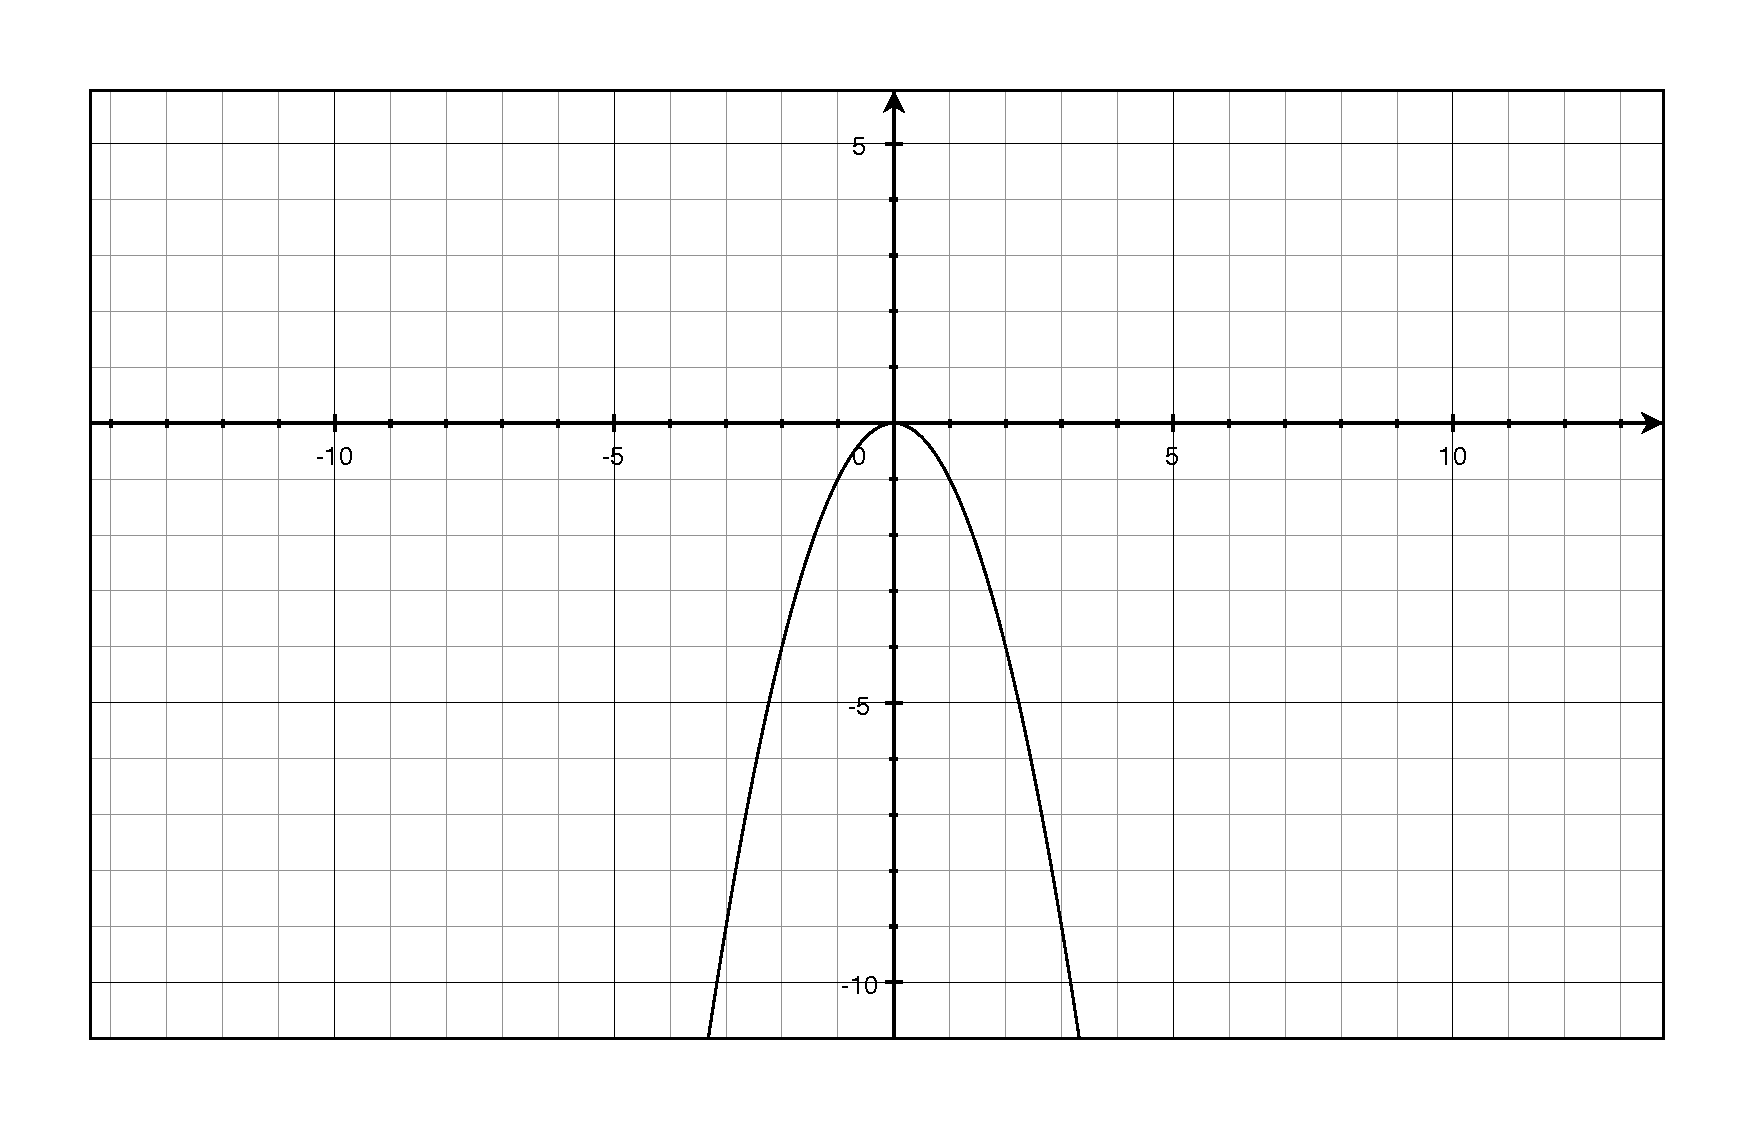
\includegraphics[scale=0.9]{problem7.eps}
%   \caption*{Problem 7}
% \end{figure}

% \begin{tabular}{cc}
%   \toprule
%   period & amplitude \\
%   \midrule
%   value one & value two
%   \bottomrule
% \end{tabular}

\printanswers

\ifprintanswers 
  \usepackage{2in1, lscape} 
\fi

\date{June 5, 2013}
\author{}
\title{Math 141 \\ Homework 13}

\begin{document}

  \maketitle

  \section{Homework}

  Section 4.1: 11-12, 15-30, 33-40, 45, 64, 66-68, 73-77, 79, 81, 83

  \section{Review}

  \begin{enumerate}
    \item Simplify: $\frac{\sqrt{-4}\sqrt{-27}\sqrt{-16}}{\sqrt{-3}}$
      \begin{solution}
        \begin{align*}
          \frac{\sqrt{-4}\sqrt{-27}\sqrt{-16}}{\sqrt{-3}} &= \frac{2i \cdot 3i \sqrt{3} \cdot 4i}{i \sqrt{3}} \\
          &= \frac{24i^3 \sqrt{3}}{i \sqrt{3}} \\
          &= 24 i^2 \\
          &= -24 \\
        \end{align*}
      \end{solution}

    \item
      \[
        f(x) = -2x^2 - 8x - 15
      \]

      \begin{parts}
        \part Express $f$ in standard form (Section 2.5)
        \begin{solution}

          \begin{align*}
            f(x)             &= - 2x^2 - 8x - 15
            - \frac{f(x)}{2} &= x^2 + 4x + \frac{15}{2} \\
                             &= x^2 + 4x + 4 - 4 + \frac{15}{2} \\
                             &= (x + 2)^2 + \frac{7}{2} \\
            f(x)             &= \boxed{- 2 (x + 2)^2 - 7} \\
          \end{align*}
          
        \end{solution}
        
      \end{parts}

  \end{enumerate}


  \section{Extra Credit}
  Section 4.1, problems 49 and 50

  \ifprintanswers
    \begin{description}
      \item[49]
        \begin{align*}
          \cosh^2(x) &- \sinh^2(x) \\
                     &= \left( \frac{e^x + e^{-x}}{2} \right)^2 - \left( \frac{e^x - e^{-x}}{2} \right)^2 \\
                     &= \frac{e^{2x} + 2 + e^{-2x}}{4} - \frac{e^{2x} - 2 + e^{-2x}}{4} \\
                     &= \frac{4}{4} \\
                     &= 1 \\
        \end{align*}

      \item[50]
        For this one you have to start from the right side:
        \begin{align*}
          \sinh(x) & \cosh(y) + \cosh(x) \sinh(y) \\
                            &= \frac{e^x - e^{-x}}{2} \cdot \frac{e^y + e^{-y}}{2} 
                                 + \frac{e^x + e^{-x}}{2} \cdot \frac{e^y - e^{-y}}{2} \\
                            &= \frac{e^{x + y} + e^{x - y} - e^{y - x} - e^{-x - y}}{4} 
                                + \frac{e^{x + y} - e^{x - y} + e^{y - x} - e^{-x - y}}{4} \\
                            &= \frac{2e^{x + y} - 2e^{-x - y}}{4} \\
                            &= \frac{e^{x + y} - e^{-(x + y)}}{2} \\
                            &= \sinh(x + y) \\
        \end{align*}
        
    \end{description}


    \section{Section 4.1}

    \begin{description}

      \item[11] 
        \begin{figure}[H]
          \centering
          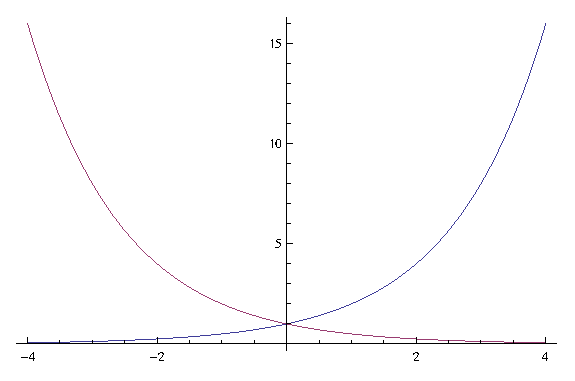
\includegraphics[scale=0.9]{exercise11.eps}
          \caption*{Exercise 11}
        \end{figure}

      \item[12] 
        \begin{figure}[H]
          \centering
          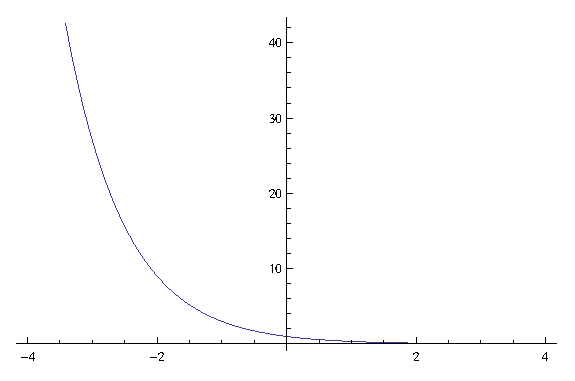
\includegraphics[scale=0.9]{exercise12.eps}
          \caption*{Exercise 12}
        \end{figure}

      \item[15] $f(x) = 3^x$

      \item[16] $f(x) = 5^x$

      \item[17] $f(x) = 4^{-x}$

      \item[18] $f(x) = 2^{-x}$

      \item[19] III

      \item[20] V

      \item[21] I

      \item[22] VI

      \item[23] II

      \item[24] IV

      \item[25] 
        \begin{figure}[H]
          \centering
          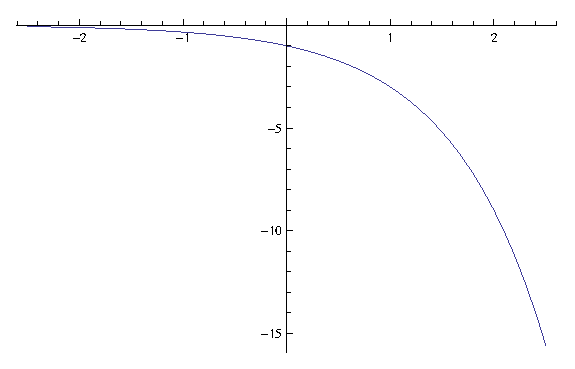
\includegraphics[scale=0.9]{exercise25.eps}
          \caption*{Exercise 25: $f(x) = -3^x$}
        \end{figure}

        \begin{tabular}[H]{ll}
          \toprule
          domain    & $(-\infty, \infty)$ \\
          range     & $(-\infty, 0)$ \\
          asymptote & $y = 0$ \\
          \bottomrule
        \end{tabular}

      \item[26] 
        \begin{figure}[H]
          \centering
          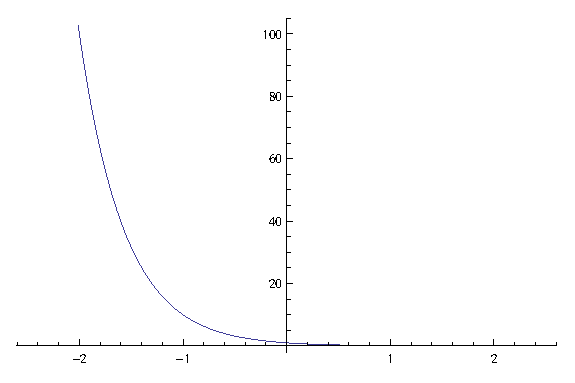
\includegraphics[scale=0.9]{exercise26.eps}
          \caption*{Exercise 26: $f(x) = 10^{-x}$}
        \end{figure}

        \begin{tabular}[H]{ll}
          \toprule
          domain    & $(-\infty, \infty)$ \\
          range     & $(0, \infty)$ \\
          asymptote & $y = 0$ \\
          \bottomrule
        \end{tabular}

      \item[27] 
        \begin{figure}[H]
          \centering
          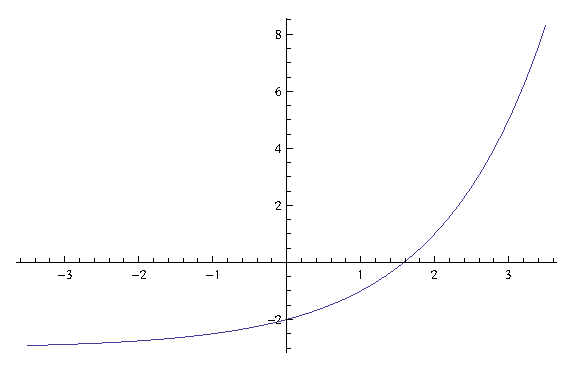
\includegraphics[scale=0.9]{exercise27.eps}
          \caption*{Exercise 27: $g(x) = 2^x - 3$}
        \end{figure}

        \begin{tabular}[H]{ll}
          \toprule
          domain    & $(-\infty, \infty)$ \\
          range     & $(-3, \infty)$ \\
          asymptote & $y = -3$ \\
          \bottomrule
        \end{tabular}

      \item[28] 
        \begin{figure}[H]
          \centering
          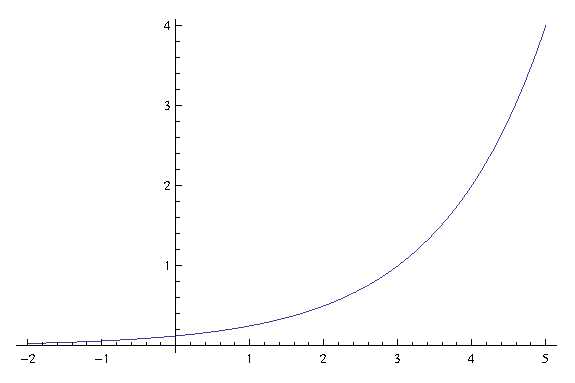
\includegraphics[scale=0.9]{exercise28.eps}
          \caption*{Exercise 28: $g(x) = 2^{x - 3}$}
        \end{figure}

        \begin{tabular}[H]{ll}
          \toprule
          domain    & $(-\infty, \infty)$ \\
          range     & $(0, \infty)$ \\
          asymptote & $y = 0$ \\
          \bottomrule
        \end{tabular}

      \item[29] 
        \begin{figure}[H]
          \centering
          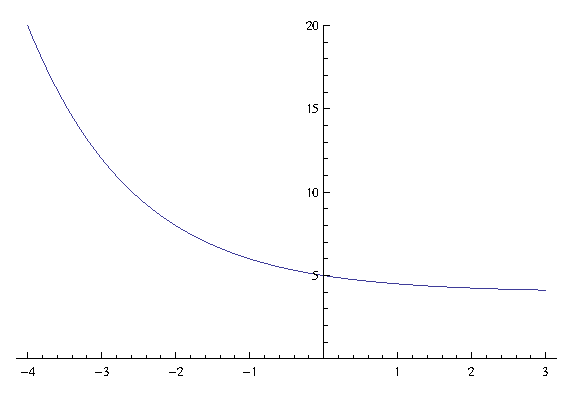
\includegraphics[scale=0.9]{exercise29.eps}
          \caption*{Exercise 29: $g(x) = 4 + \left( \frac{1}{2} \right)^x$}
        \end{figure}

        \begin{tabular}[H]{ll}
          \toprule
          domain    & $(-\infty, \infty)$ \\
          range     & $(4, \infty)$ \\
          asymptote & $y = 4$ \\
          \bottomrule
        \end{tabular}

      \item[30] 
        \begin{figure}[H]
          \centering
          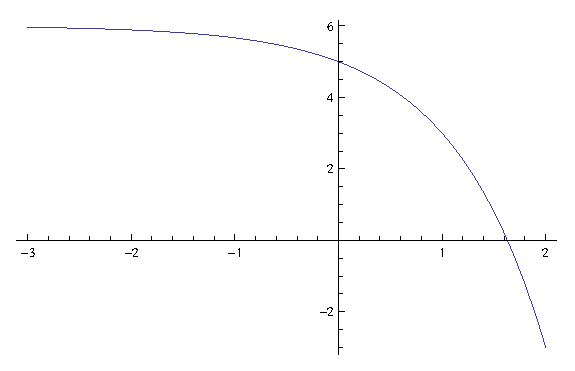
\includegraphics[scale=0.9]{exercise30.eps}
          \caption*{Exercise 30: $g(x) = 6 - 3^x$}
        \end{figure}

        \begin{tabular}[H]{ll}
          \toprule
          domain    & $(-\infty, \infty)$ \\
          range     & $(-\infty, 6)$ \\
          asymptote & $y = 6$ \\
          \bottomrule
        \end{tabular}

      \item[33] 
        \begin{figure}[H]
          \centering
          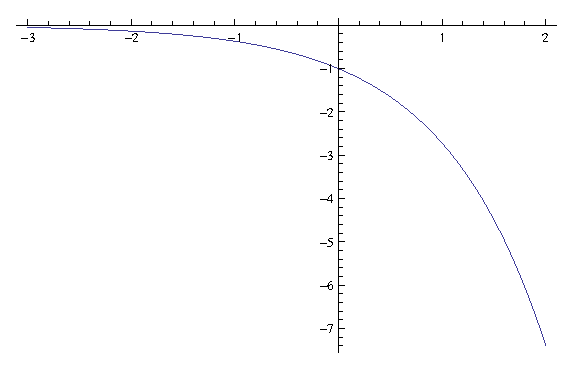
\includegraphics[scale=0.9]{exercise33.eps}
          \caption*{Exercise 33: $g(x) = -e^x$}
        \end{figure}

        \begin{tabular}[H]{ll}
          \toprule
          domain    & $(-\infty, \infty)$ \\
          range     & $(-\infty, 0)$ \\
          asymptote & $y = 0$ \\
          \bottomrule
        \end{tabular}

      \item[34] 
        \begin{figure}[H]
          \centering
          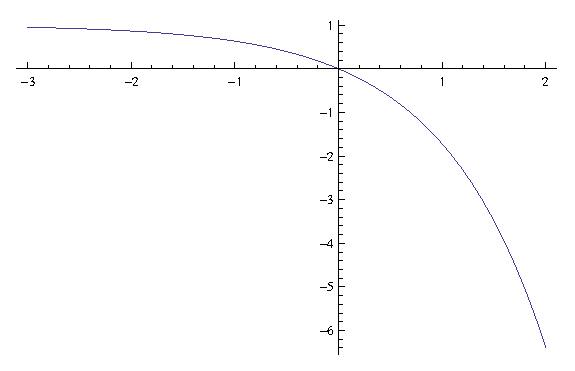
\includegraphics[scale=0.9]{exercise34.eps}
          \caption*{Exercise 34: $g(x) = 1 - e^x$}
        \end{figure}

        \begin{tabular}[H]{ll}
          \toprule
          domain    & $(-\infty, \infty)$ \\
          range     & $(-\infty, 1)$ \\
          asymptote & $y = 1$ \\
          \bottomrule
        \end{tabular}

      \item[35] 
        \begin{figure}[H]
          \centering
          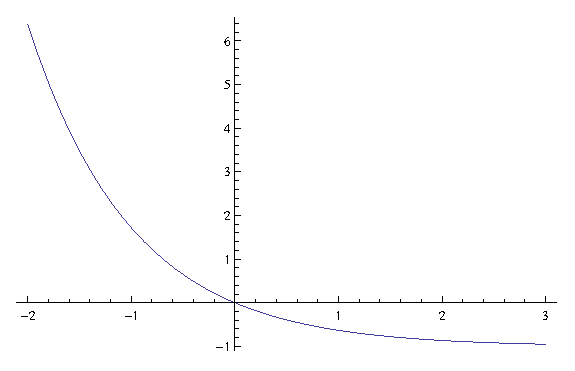
\includegraphics[scale=0.9]{exercise35.eps}
          \caption*{Exercise 35: $g(x) = e^{-x} - 1$}
        \end{figure}

        \begin{tabular}[H]{ll}
          \toprule
          domain    & $(-\infty, \infty)$ \\
          range     & $(-\infty, -1)$ \\
          asymptote & $y = -1$ \\
          \bottomrule
        \end{tabular}

      \item[36] 
        \begin{figure}[H]
          \centering
          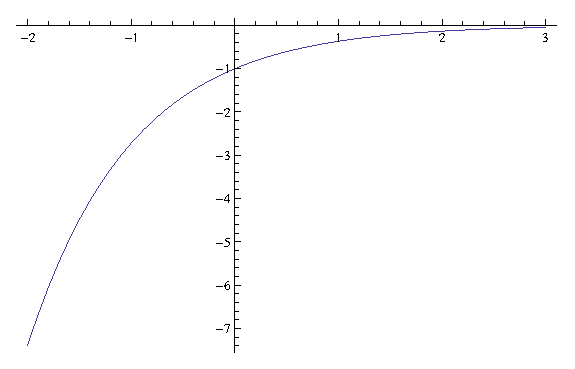
\includegraphics[scale=0.9]{exercise36.eps}
          \caption*{Exercise 36: $g(x) = -e^{-x}$}
        \end{figure}

        \begin{tabular}[H]{ll}
          \toprule
          domain    & $(-\infty, \infty)$ \\
          range     & $(-\infty, 0)$ \\
          asymptote & $y = 0$ \\
          \bottomrule
        \end{tabular}

      \item[37] 
        \begin{figure}[H]
          \centering
          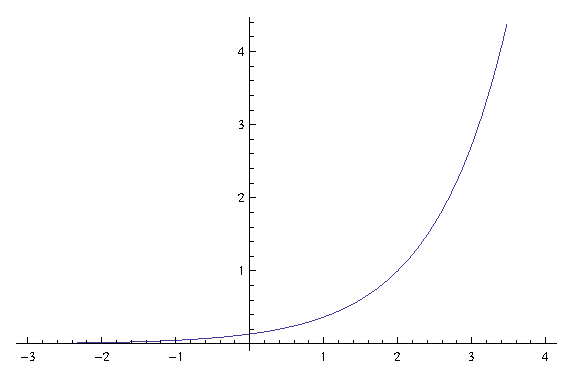
\includegraphics[scale=0.9]{exercise37.eps}
          \caption*{Exercise 37: $g(x) = e^{x - 2}$}
        \end{figure}

        \begin{tabular}[H]{ll}
          \toprule
          domain    & $(-\infty, \infty)$ \\
          range     & $(0, \infty)$ \\
          asymptote & $y = 0$ \\
          \bottomrule
        \end{tabular}

      \item[38] 
        \begin{figure}[H]
          \centering
          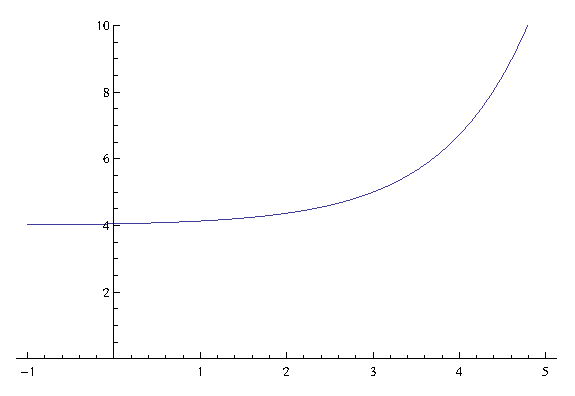
\includegraphics[scale=0.9]{exercise38.eps}
          \caption*{Exercise 38: $g(x) = e^{x - 3} + 4$}
        \end{figure}

        \begin{tabular}[H]{ll}
          \toprule
          domain    & $(-\infty, \infty)$ \\
          range     & $(4, \infty)$ \\
          asymptote & $y = 4$ \\
          \bottomrule
        \end{tabular}

      \item[39]
        The first point provides the constant:
        \begin{align*}
          Ca^0 &= 3 \\
          C    &= 3 \\
        \end{align*}

        Now we have the constant, the second point provides the base:
        \begin{align*}
          3a^2 &= 12 \\
          a^2  &= 4 \\
          a    &= 2 \\
        \end{align*}

        The function is: $f(x) = 3 \cdot 2^x$

      \item[40]
        The first point provides the constant:
        \begin{align*}
          Ca^0 &= 5 \\
          C    &= 5 \\
        \end{align*}

        Now we have the constant, the second point provides the base:
        \begin{align*}
          5a^{-1}     &= 15 \\
          \frac{1}{a} &= 3 \\
          a           &= \frac{1}{3} \\
        \end{align*}

        The function is: $f(x) = 5 \left( \frac{1}{3} \right)^x$ or $f(x) = 5 \cdot 3^{-x}$

      \item[45] 
        \begin{figure}[H]
          \centering
          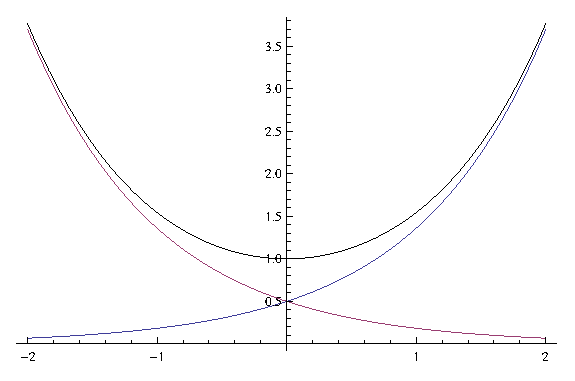
\includegraphics[scale=0.9]{exercise45.eps}
          \caption*{Exercise 45: $f(x) = \cosh(x)$}
        \end{figure}

        This is the shape a dangling chain makes when it is only supported at its ends.  It is also the shape of the
        Gateway Arch in St. Louis (upside down, of course).

      \item[64] $D(3) 50 e^{-0.2 \cdot 3} \approx \unit[27.4066]{mg}$

      % \item[65]
      %   \begin{enumerate}[a]
      %     \item $m(0) = 13$
      %     \item $m(45) \approx 0.0152214$
      %   \end{enumerate}

      \item[66]
        \begin{enumerate}[a]
          \item $m(0) = \unit[6]{kg}$
          \item $m(20) \approx \unit[1.05312]{kg}$
        \end{enumerate}

      \item[67]
        \begin{enumerate}[a]
          \item $f(0) = \unit[0]{ft/s}$

          \item $f(5) \approx \unit[50.6]{ft/s}$; $f(10) \approx \unit[69.2]{ft/s}$

          \item
            \begin{figure}[H]
              \centering
              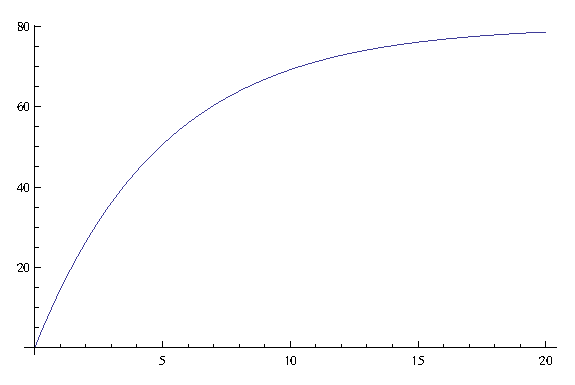
\includegraphics[scale=0.9]{exercise67.eps}
              \caption*{Exercise 67: $f(x) = 80 \left( 1 - e^{-0.2t} \right)$}
            \end{figure}

          \item As $t$ gets larger and larger, the velocity gets closer and closer to $\unit[80]{f/s}$, so this is the
            terminal velocity.

        \end{enumerate}

      \item[68]
        \begin{enumerate}[a]
          \item $P(0) = 100$

          \item
            \begin{tabular}[H]{lr}
              \toprule
              year & population \\
              \midrule
              10   & 482 \\
              20   & 999 \\
              30   & 1,168 \\
              \bottomrule
            \end{tabular}

          \item As time goes by the denominator approaches 1 and the number of fish approaches 1,200 which agrees with
            the graph.

        \end{enumerate}

      \item[73]
        \begin{tabular}[H]{lr}
          \toprule
          year & amount \\
          \midrule
          1    & \$5,203.71 \\
          2    & \$5,415.71 \\
          3    & \$5,636.36 \\
          4    & \$5,865.99 \\
          5    & \$6,104.98 \\
          6    & \$6,353.71 \\
          \bottomrule
        \end{tabular}

      \item[74]
        \begin{tabular}[H]{lr}
          \toprule
          rate & amount \\
          \midrule
          1\% & \$5,256.25 \\
          2\% & \$5,525.39 \\
          3\% & \$5,808.08 \\
          4\% & \$6,104.98 \\
          5\% & \$6,416.79 \\
          6\% & \$6,744.25 \\
          \bottomrule
        \end{tabular}

      \item[75]
        \begin{tabular}[H]{lr}
          \toprule
          year & amount \\
          \midrule
          5    & \$16,288.90 \\
          10   & \$26,533.00 \\
          15   & \$43,219.40 \\
          \bottomrule
        \end{tabular}

      \item[76]
        \begin{tabular}[H]{lr}
          \toprule
          year & amount \\
          \midrule
          4    & \$7,491.92 \\
          6    & \$10,253.20 \\
          8    & \$14,032.20 \\
          \bottomrule
        \end{tabular}

      \item[77]
        \begin{tabular}[H]{lr}
          \toprule
          compounding  & amount \\
          \midrule
          annually     & \$4,615.87 \\
          semiannually & \$4,658.91 \\
          monthly      & \$4,697.04 \\
          weekly       & \$4,686.14 \\
          daily        & \$4,704.68 \\
          hourly       & \$4,704.93 \\
          continuously & \$4,704.94 \\
          \bottomrule
        \end{tabular}

      \item[79]
        \begin{enumerate}[i]
          \item $P \left( 1 + \frac{.085}{2} \right)^{2t} = P 1.08681^t$.  This is the best deal.
          \item $P \left( 1 + \frac{.0825}{4} \right)^{4t} = P 1.08509^t$
          \item $P e^{.08t} = P 1.08329 t$
        \end{enumerate}

      \item[81]
        \begin{enumerate}[a]
          \item 
            \begin{align*}
              10,000 &= P  \left( 1 + \frac{0.09}{2} \right)^{2 \cdot 3} \\
              P      &= 7,678.96 \\
            \end{align*}

          \item 
            \begin{align*}
              100,000 &= P  \left( 1 + \frac{0.08}{12} \right)^{12 \cdot 5} \\
              P       &= 67,121 \\
            \end{align*}
        \end{enumerate}

      \item[83]
        When you are paid by the daily scheme, the amount of money you have after each day is:

        \begin{tabular}[H]{lr}
          \toprule
          day  & total (cents) \\
          \midrule
          1 & $2$ \\
          2 & $2 + 4 = 6$ \\
          3 & $2 + 4 + 8 = 14$ \\
          4 & $2 + 4 + 8 + 16 = 30$ \\
          5 & $2 + 4 + 8 + 16 + 32 = 62$ \\
          n & $2^{n + 1} - 2$ \\
          \bottomrule
        \end{tabular}

        Using the general formula, after day 30, you'll have made:
        \[
          2^{31} - 2 = \unit[2,147,483,646]{cents} = \$21,474,836.46
        \]

        which is much better than the measely million you'd get with the other plan.
    \end{description}

  \else
    \vspace{6 cm}
    \begin{quote}
      \begin{em}
        Most of the luxuries, and many of the so-called comforts of life, are not only not indispensable, but positive
        hindrances to the elevation of mankind.  
      \end{em}
    \end{quote}

    \hspace{1 cm} --Henry David Thoreau
  \fi

\end{document}

